\documentclass[conference]{IEEEtran}
\usepackage{amsmath}
\usepackage{booktabs}
\usepackage{cite}
\usepackage{url}
\usepackage{tikz}
\usepackage{pgfplots}
\usetikzlibrary{arrows.meta,positioning,shapes.geometric}
\pgfplotsset{compat=1.18}

\title{RansomShield: A Behavioral Machine Learning Framework\\
for Decoy-Server Ransomware Activity Monitoring and Alerting}

\author{
\IEEEauthorblockN{Archana M, Chandan T. N., Gouri K. Patil, and Karan S.}
\IEEEauthorblockA{Department of Computer Science and Engineering\\
Bapuji Institute of Engineering and Technology, Davanagere, India\\
Project Guide: Dr. Usha G. R.}
}

\begin{document}
\maketitle

\begin{abstract}
Ransomware can cause significant damage between the beginning of abnormal file
activity and the response of a conventional signature-based defense. This paper
presents RansomShield, a safe behavioral monitoring and alerting prototype that
combines file-system change signals, host resource telemetry, and interaction
with synthetic canary assets on an isolated decoy server. The system is
implemented as a modular Flask application with authenticated access, protected
application programming interfaces, a background monitoring service, persistent
SQLite evidence, and a responsive dashboard. A hybrid temporal convolutional
network (TCN) and XGBoost classifier estimates suspicious-activity probability
from eight-window sequences of eleven behavioral features. The TCN extracts a
causal temporal representation, which XGBoost combines with the latest engineered
feature vector. A reproducible experiment using 6,000 synthetic sequences achieved
96.92\% held-out accuracy and a 96.51\% F1-score. These values validate software and model
integration only; they do not establish performance against real ransomware. The
prototype therefore provides a controlled foundation for future evaluation using
labeled endpoint traces.
\end{abstract}

\begin{IEEEkeywords}
ransomware detection, behavioral monitoring, honeypot, decoy server, canary files,
temporal convolutional network, XGBoost, cybersecurity, machine learning
\end{IEEEkeywords}

\section{Introduction}
Ransomware denies access to data, commonly by encrypting or otherwise modifying
large collections of files. Signature-based detection remains useful for known
families, but unseen variants and rapidly changing samples motivate observation
of behavior in addition to static identity. Repeated file modifications,
deletions, resource-use changes, and unusual process activity can provide early
indicators of destructive behavior. Prior systems such as CryptoDrop have shown
the value of monitoring file transformations while limiting data loss
\cite{scaife2016cryptodrop}. Broader ransomware studies similarly emphasize the
importance of understanding run-time behavior rather than relying on names or
extensions alone \cite{kharraz2015gordian}.

RansomShield explores this direction through a bounded, demonstrable application.
It does not execute malware, inspect arbitrary personal directories, terminate
processes, or claim production-grade protection. Instead, it watches an isolated
synthetic server with Finance, HR, Backup, and Documents assets, collects an
eleven-value telemetry vector every two seconds, applies a
trained probability model, and presents evidence through a protected dashboard.
This safe scope supports repeatable classroom and research demonstrations.

The principal contributions are:
\begin{itemize}
    \item an end-to-end architecture joining safe host monitoring, model
    inference, persistent evidence, alerts, and an authenticated web interface;
    \item a safe decoy-server hierarchy with attractive dummy assets and three
    canary files that add early-warning evidence without exposing real data;
    \item a causal TCN feature extractor and XGBoost classifier with model schema
    validation and a deterministic heuristic fallback;
    \item a reproducible sequential synthetic-data training procedure and
    held-out XGBoost-only ablation; and
    \item an explicit separation between demonstrated prototype results and the
    real-endpoint validation required for future claims.
\end{itemize}

\section{Related Work}
Behavioral ransomware research has examined file access patterns, content
transformations, decoy resources, and system-level events. Kharraz \emph{et al.}
analyzed ransomware behavior and discussed practical defensive opportunities
\cite{kharraz2015gordian}. Scaife \emph{et al.} proposed CryptoDrop, an early-warning
system based on suspicious file changes \cite{scaife2016cryptodrop}. These works
motivate RansomShield's use of created, modified, and deleted file counts.

Machine-learning classifiers provide a way to combine several weak behavioral
signals. Temporal convolutional networks (TCNs) model ordered observations with
causal convolutions \cite{bai2018tcn}, while XGBoost provides efficient nonlinear
boosted-tree classification \cite{chen2016xgboost}. RansomShield combines these
methods: the TCN summarizes recent telemetry and XGBoost fuses that representation
with the latest engineered measurements. This retains explicit behavioral inputs
while introducing temporal context.

\section{System Requirements and Threat Model}
The prototype targets bursts of suspicious activity observable through aggregated
file-system and resource measurements. An authenticated user can start or stop
the monitor, generate harmless demonstration files, inspect recent events and
alerts, and acknowledge reviewed alerts. The monitored scope is restricted to
\texttt{instance/decoy\_server}; every contained asset is synthetic.

The threat model assumes that suspicious activity produces at least one measured
behavioral change during a polling window. The current system does not defend
against kernel-level attackers, telemetry tampering, slow ``low-and-slow''
activity designed to remain below thresholds, or activity outside the configured
directory. Snapshot polling reliably observes canary modification or removal,
but cannot claim read-only access detection; production deployment would require
operating-system audit telemetry or an endpoint agent. High-risk detections now
support file quarantine within the synthetic monitored scope; this file move does
not terminate the responsible process or provide decryption or recovery.

\section{Architecture and Implementation}
RansomShield uses a modular Flask architecture. Flask-Login manages sessions;
Flask-WTF supplies cross-site request forgery protection; SQLAlchemy maps users,
monitoring events, and alerts to SQLite; and \texttt{psutil} reads CPU, memory,
and process information. Passwords are stored as salted hashes rather than plain
text. Dashboard and monitoring routes require an authenticated session, and
state-changing routes use HTTP POST requests.

The processing pipeline is:
\begin{equation}
\text{Snapshot} \rightarrow \text{Feature Extraction} \rightarrow
\text{ML Inference} \rightarrow \text{Event/Alert} \rightarrow \text{Dashboard}.
\end{equation}

Fig.~\ref{fig:architecture} summarizes the separation between telemetry
collection, inference, persistence, protected services, and presentation.

\begin{figure*}[t]
\centering
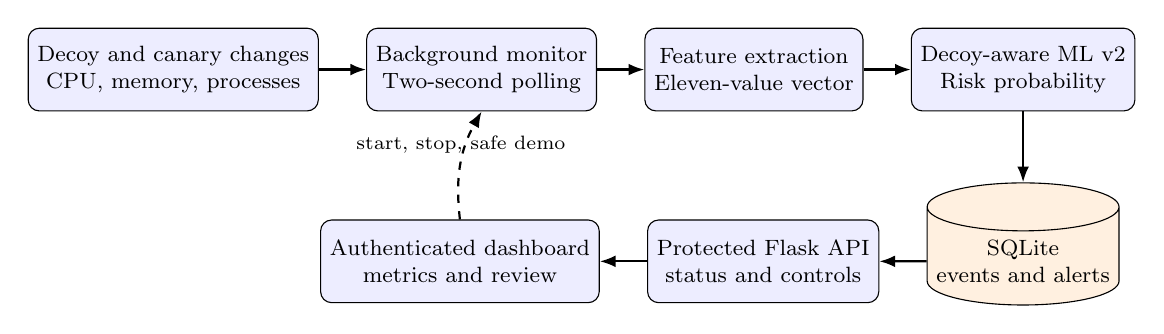
\begin{tikzpicture}[
node distance=7mm and 6mm,
block/.style={draw,rounded corners,minimum width=2.55cm,minimum height=1.05cm,
align=center,font=\footnotesize,fill=blue!7},
data/.style={draw,cylinder,shape border rotate=90,aspect=0.25,minimum width=2.15cm,
minimum height=1.15cm,align=center,font=\footnotesize,fill=orange!12},
arrow/.style={-{Latex[length=2mm]},thick}]
\node[block] (inputs) {Decoy and canary changes\\CPU, memory, processes};
\node[block,right=of inputs] (monitor) {Background monitor\\Two-second polling};
\node[block,right=of monitor] (features) {Feature extraction\\Eleven-value vector};
\node[block,right=of features] (model) {Decoy-aware ML v2\\Risk probability};
\node[data,below=9mm of model] (db) {SQLite\\events and alerts};
\node[block,left=of db] (api) {Protected Flask API\\status and controls};
\node[block,left=of api] (ui) {Authenticated dashboard\\metrics and review};
\draw[arrow] (inputs) -- (monitor);
\draw[arrow] (monitor) -- (features);
\draw[arrow] (features) -- (model);
\draw[arrow] (model) -- (db);
\draw[arrow] (db) -- (api);
\draw[arrow] (api) -- (ui);
\draw[arrow,dashed] (ui.north) to[bend left=18]
node[above,font=\scriptsize]{start, stop, safe demo} (monitor.south);
\end{tikzpicture}
\caption{RansomShield end-to-end architecture. Monitoring is bounded to an
isolated synthetic server; control endpoints require authentication.}
\label{fig:architecture}
\end{figure*}

At monitor start, the service records each sample file's relative path,
modification time, and size. On each two-second cycle, it compares the new and
previous snapshots to count creations, modifications, and deletions. The service
then reads CPU utilization, memory utilization, and running-process count. The
eleven values form the feature vector shown in Table~\ref{tab:features}.

The run-time decision sequence is illustrated in Fig.~\ref{fig:workflow}. A
cycle with no file change updates live metrics without creating database noise;
observed activity is scored and preserved for review.

\begin{figure}[t]
\centering
\begin{tikzpicture}[
node distance=4mm,
step/.style={draw,rounded corners,minimum width=3.1cm,minimum height=6mm,
align=center,font=\scriptsize,fill=green!7},
decision/.style={draw,diamond,aspect=2.6,align=center,font=\scriptsize,fill=yellow!12},
arrow/.style={-{Latex[length=1.7mm]},thick}]
\node[step] (snap) {Read snapshot and telemetry};
\node[step,below=of snap] (diff) {Count file-system changes};
\node[decision,below=5mm of diff] (change) {File activity?};
\node[step,below left=7mm and -1mm of change] (metrics) {Update metrics};
\node[step,below right=7mm and -1mm of change] (score) {Predict risk};
\node[decision,below=7mm of score] (threshold) {Risk $\geq 60$?};
\node[step,below left=7mm and -2mm of threshold] (event) {Save event};
\node[step,below right=7mm and -2mm of threshold] (alert) {Save event\\and alert};
\draw[arrow] (snap) -- (diff);
\draw[arrow] (diff) -- (change);
\draw[arrow] (change) -| node[near start,above,font=\scriptsize]{no} (metrics);
\draw[arrow] (change) -| node[near start,above,font=\scriptsize]{yes} (score);
\draw[arrow] (score) -- (threshold);
\draw[arrow] (threshold) -| node[near start,above,font=\scriptsize]{no} (event);
\draw[arrow] (threshold) -| node[near start,above,font=\scriptsize]{yes} (alert);
\end{tikzpicture}
\caption{Monitoring and machine-learning inference workflow.}
\label{fig:workflow}
\end{figure}

\begin{table}[t]
\caption{Behavioral Model Features}
\label{tab:features}
\centering
\begin{tabular}{ll}
\toprule
Feature & Description \\
\midrule
$x_1$ & Files created in the current interval \\
$x_2$ & Files modified in the current interval \\
$x_3$ & Files deleted in the current interval \\
$x_4$ & CPU utilization percentage \\
$x_5$ & Memory utilization percentage \\
$x_6$ & Number of running processes \\
$x_7$ & Canary observably touched (binary) \\
$x_8$ & Canary modified (binary) \\
$x_9$ & Number of decoy files touched \\
$x_{10}$ & Number of top-level directories touched \\
$x_{11}$ & File operations per second \\
\bottomrule
\end{tabular}
\end{table}

The service persists a monitoring event whenever file activity occurs. A risk
score at or above 60 creates an alert; scores at or above 85 receive high
severity, while other triggered alerts receive medium severity. The database
stores event type, description, severity, score, time, acknowledgement state,
and user-account information. JSON endpoints expose status, events, and alerts
to the dashboard.

\section{Model Training and Inference}
\subsection{Safe Synthetic Dataset}
No labeled real-endpoint dataset is included in the project. To test the complete
training-to-inference path safely, a deterministic generator creates 6,000
telemetry records using random seed 20260827. Benign samples are drawn from
lower-activity distributions; suspicious samples use higher file-change and
resource-use distributions. Approximately 3.5\% of labels are flipped to add
ambiguity. The shuffled records are divided into 4,800 training samples and 1,200
held-out samples.

Synthetic generation provides repeatability and avoids distributing malware or
sensitive endpoint traces. Its distributions are designed by the developers,
however, so results can reflect those assumptions. The generated data must not
be treated as evidence of real-world ransomware detection capability.

\subsection{TCN--XGBoost Hybrid}
For each feature $x_j$, training calculates mean $\mu_j$ and standard deviation
$\sigma_j$. The standardized feature is
\begin{equation}
z_j = \frac{x_j-\mu_j}{\sigma_j}.
\end{equation}
Eight consecutive standardized telemetry vectors form the input sequence
$\mathbf{Z}\in\mathbb{R}^{8\times11}$. A causal one-dimensional convolution with
eight filters, kernel size three, and dilation two computes
\begin{equation}
h_{t,f}=\operatorname{ReLU}\!\left(b_f+\sum_{k=0}^{2}\sum_{j=1}^{11}
W_{f,k,j}z_{\max(0,t-2k),j}\right).
\end{equation}
Temporal averaging produces the eight-value representation
$e_f=\frac{1}{8}\sum_t h_{t,f}$. The convolution weights are learned for 180 epochs
using binary cross-entropy. XGBoost receives the concatenation of $\mathbf{e}$ and
the latest standardized eleven-feature vector. It uses 160 boosted trees, maximum
depth four, learning rate 0.05, and row and column subsampling of 0.9.

The model metadata stores its schema version, feature order, normalization
statistics, temporal configuration, threshold, training metadata, and metrics.
TCN weights are stored in NPZ format and the booster in XGBoost JSON format.

At startup, the application validates the model type and ordered feature names,
then loads both model artifacts. Until eight observations are available, the
earliest observation pads the left side of the causal window.
An invalid or missing artifact activates the prior explainable heuristic and
reports ``Heuristic fallback'' on the dashboard. This behavior maintains service
availability without silently presenting fallback output as ML output.

\section{Experimental Results}
Performance is calculated on the 1,200 sequences excluded from training. Accuracy,
precision, recall, and F1-score are defined in the usual manner from true
positives ($TP$), true negatives ($TN$), false positives ($FP$), and false
negatives ($FN$):
\begin{align}
\text{Precision} &= TP/(TP+FP),\\
\text{Recall} &= TP/(TP+FN),\\
F1 &= 2(\text{Precision}\cdot\text{Recall})/
(\text{Precision}+\text{Recall}).
\end{align}

\begin{table}[t]
\caption{Held-Out Synthetic Telemetry Ablation}
\label{tab:results}
\centering
\begin{tabular}{lcc}
\toprule
Metric & XGBoost only & TCN + XGBoost \\
\midrule
Accuracy & 96.92\% & 96.92\% \\
Precision & 96.78\% & 96.78\% \\
Recall & 96.23\% & 96.23\% \\
F1-score & 96.51\% & 96.51\% \\
\bottomrule
\end{tabular}
\end{table}

The ablation compares the hybrid with XGBoost using only the latest telemetry
vector. Their rounded metrics are equal on this synthetic distribution; therefore,
the experiment does not claim a measurable TCN advantage. It establishes that the
requested temporal hybrid is trained, serialized, and executed end to end. The
application successfully loaded both artifacts and reported
\texttt{TCN + XGBoost Behavioral Model} through its status interface.

Fig.~\ref{fig:metrics} compares the four held-out metrics. Their similar values
indicate balanced performance within the generated test distribution, rather
than a result dominated by only one class.

\begin{figure}[t]
\centering
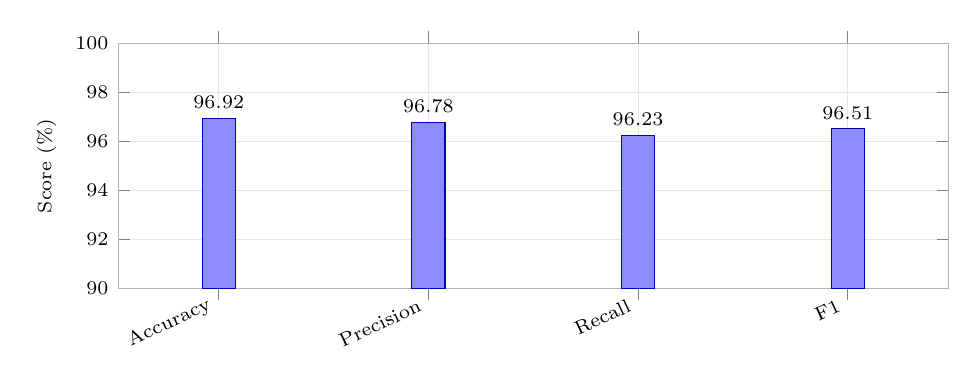
\begin{tikzpicture}
\begin{axis}[
ybar,width=\columnwidth,height=4.7cm,ymin=90,ymax=100,
ylabel={Score (\%)},symbolic x coords={Accuracy,Precision,Recall,F1},xtick=data,
x tick label style={rotate=25,anchor=east,font=\scriptsize},
y tick label style={font=\scriptsize},ylabel style={font=\scriptsize},
bar width=12pt,nodes near coords,nodes near coords style={font=\scriptsize},
grid=major,grid style={gray!20},axis line style={gray!60},enlarge x limits=0.16]
\addplot[fill=blue!45,draw=blue!70!black] coordinates {
(Accuracy,96.92) (Precision,96.78) (Recall,96.23) (F1,96.51)};
\end{axis}
\end{tikzpicture}
\caption{Held-out results on 1,200 safe synthetic telemetry sequences. The scores
validate the prototype pipeline, not real-world ransomware efficacy.}
\label{fig:metrics}
\end{figure}

These tests show that serialization, loading, feature ordering, normalization,
temporal buffering, hybrid inference, and dashboard exposure operate consistently. They do
not compare the model with commercial defenses or establish resilience against
unseen ransomware families.

\section{Security, Safety, and Limitations}
The demonstration endpoint creates harmless placeholders, appends a safe marker
to synthetic canaries, and removes disposable dummy files within the isolated
decoy directory. It neither
encrypts files nor invokes malware. Authentication,
password hashing, CSRF validation, HTTP-only cookies, same-site cookie policy,
and safe post-login redirects reduce common web risks. Deployment would still
require a strong external secret key, HTTPS, secure-cookie enforcement, database
migrations, rate limiting, per-user or per-agent data ownership, centralized
logging, and a production WSGI server.

The principal research limitation is the synthetic dataset. Because its labels
and distributions are generated from assumed behavior, the high held-out metrics
mainly show separability within that simulation. Further limitations include
two-second aggregation that may discard ordering information, monitoring of only
one directory, a single-process local monitor, no threshold calibration on a
real benign workload, and no measurement of detection latency or files lost
before alerting.

\subsection{External Evaluation and Automated Response Extensions}
The implementation includes a frozen-model CSV evaluation command that validates
the eleven input features, orders consecutive two-second windows within each
trace, and resets temporal history between traces. Its report records dataset
provenance, model and input hashes, the decision threshold, confusion counts,
accuracy, precision, recall, F1, and false-positive rate. No independent published
dataset has yet been evaluated with this extension; the numerical results in this
paper remain synthetic. Published feature matrices require a reviewed conversion
to compatible telemetry and cannot substitute missing measurements with assumed
zeros.

For alerts with risk scores of at least 85, the monitor can move affected regular
files into an alert-specific quarantine directory outside the monitored tree.
Per-file outcomes and optional HTTPS webhook or STARTTLS email delivery statuses
are persisted and exposed in the dashboard. Deleted or inaccessible files are
reported as failed moves. Quarantine-generated removals are excluded from the next
poll's change set. Notifications require operator configuration; delivery failure
does not undo containment. These actions are bounded prototype responses rather
than a guarantee of containment against an active adversary.

\section{Future Work}
Future evaluation should collect consented benign workloads and controlled traces
from isolated ransomware test environments, define leakage-resistant train and
test partitions by family and host, and document class balance and label policy.
Required measures include receiver-operating-characteristic and
precision--recall curves, false positives per hour, calibration error, detection
latency, and the number of modified files before detection.

The present TCN--XGBoost hybrid should next be retrained on representative traces
and compared against simpler classifiers and deterministic heuristics through
ablation studies. Production work should add authenticated
endpoint agents, signed telemetry, per-agent ownership, model-version tracking,
drift monitoring, and carefully governed response actions.

\section{Conclusion}
RansomShield demonstrates an end-to-end behavioral monitoring architecture rather
than a stand-alone notebook model. It safely collects bounded file and resource
telemetry, executes a trained classifier, persists evidence, produces alerts,
and exposes results through an authenticated Flask dashboard. The held-out
synthetic results verify the integration baseline, while the explicit limitations
prevent them from being confused with real-world efficacy. The project provides
a reproducible foundation for representative data collection, temporal modeling,
formal evaluation, and eventual endpoint deployment.

\begin{thebibliography}{00}
\bibitem{kharraz2015gordian}
A. Kharraz, W. Robertson, D. Balzarotti, L. Bilge, and E. Kirda,
``Cutting the Gordian knot: A look under the hood of ransomware attacks,''
in \emph{Proc. 12th Int. Conf. Detection of Intrusions and Malware, and
Vulnerability Assessment (DIMVA)}, 2015, pp. 3--24.

\bibitem{scaife2016cryptodrop}
N. Scaife, H. Carter, P. Traynor, and K. R. B. Butler,
``CryptoLock (and Drop It): Stopping ransomware attacks on user data,''
in \emph{Proc. IEEE 36th Int. Conf. Distributed Computing Systems (ICDCS)},
2016, pp. 303--312.

\bibitem{bai2018tcn}
S. Bai, J. Z. Kolter, and V. Koltun,
``An empirical evaluation of generic convolutional and recurrent networks for
sequence modeling,'' \emph{arXiv preprint arXiv:1803.01271}, 2018.

\bibitem{chen2016xgboost}
T. Chen and C. Guestrin, ``XGBoost: A scalable tree boosting system,''
in \emph{Proc. 22nd ACM SIGKDD Int. Conf. Knowledge Discovery and Data Mining},
2016, pp. 785--794.
\end{thebibliography}

\end{document}
